% IEEE conference paper. Compile with pdflatex (IEEEtran.cls ships with TeX Live and Overleaf):
%   pdflatex paper && pdflatex paper
% Figures are read from ../figures and ../../figures (docs/paper/figures, docs/figures).
% Every number is copied from docs/RESULTS.md or docs/results/*.json.
\documentclass[conference]{IEEEtran}
\usepackage[utf8]{inputenc}
\usepackage[T1]{fontenc}
\usepackage{graphicx}
\usepackage{booktabs}
\usepackage{amsmath}
\usepackage{url}
\usepackage{xcolor}
\usepackage{makecell}
\graphicspath{{../figures/}{../../figures/}}
\newcommand{\verify}{\textcolor{red}{[verify]}}

\begin{document}

\title{Do Verification Stages Reduce CCTV False Alarms Without Losing Events? An End-to-End Ablation of a Multi-Event Industrial Surveillance Pipeline}

\author{\IEEEauthorblockN{Sanchi Gangurde}
\IEEEauthorblockA{\textit{[department, institute, city, India --- verify]}\\
aimms.pid4@gmail.com}}

\maketitle

\begin{abstract}
Automatic CCTV incident detection is only useful if its alarms are trusted, and trust is lost through false alarms per hour of ordinary footage, a quantity rarely measured. We study a multi-event industrial pipeline (fight, fall, fire/smoke, unusual activity) to which four training-free verification stages were added: $N$-of-$M$ temporal persistence, a track-level interaction check for fights, a region-dynamics check for fire and smoke, and per-camera calibration of an anomaly threshold. We ablate each stage end to end, replaying 472 clips in real time through the unchanged production pipeline, and report bootstrap 95\,\% confidence intervals. The deployment-camera recordings were unavailable, so the study uses held-out and public clips as a labelled proxy. Together the stages cut false alarms on fire look-alike scenes from 109.5 to 44.6 per hour, but on normal clips only from 157.9 to 135.3 per hour (the paired interval touches zero), and they lower fight recall from 0.78 to 0.47. Per stage, persistence and anomaly calibration remove most false alarms. The fight interaction check costs 0.28 recall for a marginal gain, calibration also silenced the anomaly detector on genuine events, and region dynamics had no measurable effect. The claim that verification reduces false alarms while keeping recall holds only in part. We report what each stage costs and what remains to be measured on site.
\end{abstract}

\begin{IEEEkeywords}
video surveillance, false alarms, fight detection, fire detection, fall detection, anomaly detection, ablation study, industrial safety
\end{IEEEkeywords}

\section{Introduction}
Factories record CCTV continuously, but nobody watches every camera. Automatic incident detection can close that gap only if staff trust its alerts. A detector with a 1\,\% per-window false-positive rate, evaluated ten times a second on several cameras, still produces many false alerts per hour. After enough false alerts, operators stop responding. Published detectors are usually evaluated on curated, trimmed clips with balanced classes. The measure that decides whether a deployed system is used is different: \emph{false alarms per hour of ordinary footage, at a recall that still catches genuine events}.

We built a multi-event CCTV pipeline for a manufacturing ERP that detects fights (R3D-18~\cite{tran2018}), falls (YOLOv8-Pose~\cite{yolov8,maji2022} with a temporal CNN and BiGRU~\cite{cho2014}), fire and smoke (fine-tuned YOLOv8n~\cite{redmon2016,yolov8} with a learned verifier) and unusual activity (an optical-flow autoencoder, after~\cite{hasan2016}). On a real test camera, normal activity produced fight, smoke and ``unusual activity'' alerts every few minutes. The failures had distinct causes: a clip classifier scoring people who merely stood close together, static orange objects passing a fire detector, and an anomaly threshold learned on another site's footage. Instead of retraining, we added cheap verification stages that use evidence the detectors ignore.

\textbf{Research question.} Does a multi-stage verification pipeline (temporal persistence, track-level interaction validation for fights, a region-dynamics check for fire and smoke, and per-camera anomaly calibration) reduce false alarms per hour on normal footage while keeping recall on genuine events, and what does each stage contribute?

\textbf{Contributions.}
\begin{itemize}
\item A \textbf{verification pipeline} of four training-free stages placed after the per-event models (Fig.~\ref{fig:pipeline}), each aimed at a specific failure: single-window spikes, people who are merely close, static fire look-alikes, and a threshold from another site.
\item An \textbf{ablation protocol on the unchanged live pipeline}: every clip is replayed separately in real time through the production code. Configurations differ only in existing configuration flags, or, for the pre-verification baseline, in the code version. Results are reported as false alarms per hour and clip-level recall, with bootstrap confidence intervals.
\item \textbf{Per-stage evidence, including negative results}, on 472 held-out and public clips (a proxy: the deployment-camera recordings were unavailable). Persistence and calibration remove most false alarms; the interaction check costs more fight recall than it saves; calibration can silence the detector it calibrates; region dynamics is not exercised by public look-alikes. Every number is generated by a script from stored per-clip outcomes or metrics files.
\end{itemize}

\section{Related Work}
\textbf{Detection and tracking.} Single-stage detectors from YOLO~\cite{redmon2016} to the anchor-free Ultralytics YOLOv8~\cite{yolov8} give real-time person detection. ByteTrack~\cite{zhang2022} also associates low-confidence boxes, which reduces identity switches under occlusion. Our interaction check depends on such stable track identities.

\textbf{Violence and fight detection.} Spatio-temporal 3D CNNs~\cite{tran2018} pretrained on Kinetics~\cite{kay2017} are the standard backbone for clip-level action classification. Surveillance fight datasets~\cite{cheng2021,akti2019}~\verify{} show that clip-level spatio-temporal models outperform per-frame detection for violence. These works report clip accuracy on trimmed datasets. They do not address what a clip classifier does on hours of untrimmed footage from a camera it was not trained on, which is where our false alarms came from. Grad-CAM~\cite{selvaraju2017} explains such models; we attach Grad-CAM maps to fight alerts as evidence for the human reviewer.

\textbf{Fire and smoke.} Colour models of flame pixels~\cite{celik2009} and spatio-temporal flicker and dynamic-texture features~\cite{dimitropoulos2015}~\verify{} separate flames from flame-coloured objects. We use the same principle, that real flames and smoke \emph{change}, as a verification stage after a learned detector.

\textbf{Falls.} Pose estimation in a single-stage detector~\cite{maji2022} provides skeletons; recurrent models such as the GRU~\cite{cho2014} classify their temporal evolution.

\textbf{Anomaly detection.} Autoencoders trained on normal video flag high reconstruction error as abnormal~\cite{hasan2016}. Weakly supervised methods on UCF-Crime~\cite{sultani2018} show how hard the problem is on real surveillance footage. A threshold learned on training footage need not transfer to a new camera; we calibrate it per camera.

\textbf{Gap.} Most work studies one event type on curated data and reports per-clip metrics. A deployed system combines several event types on one stream, and its users experience false alarms per hour. Within the literature surveyed here, we are not aware of an ablation of post-hoc verification stages measured end to end through a live pipeline.

\section{Method}
Frames are processed at 10 frames/s at $640\times480$. YOLOv8n detects people, and ByteTrack assigns track IDs whose box histories are kept in a 30-s buffer. Four learned detectors read frames and tracks. Their outputs pass through the verification stages and then an event-confirmation stage with PROBABLE and CONFIRMED tiers and de-duplication (one incident per ongoing event per camera). Only CONFIRMED incidents, or PROBABLE ones later escalated, reach the dashboard; we call these \emph{alarms}.

\begin{figure*}[t]
\centering
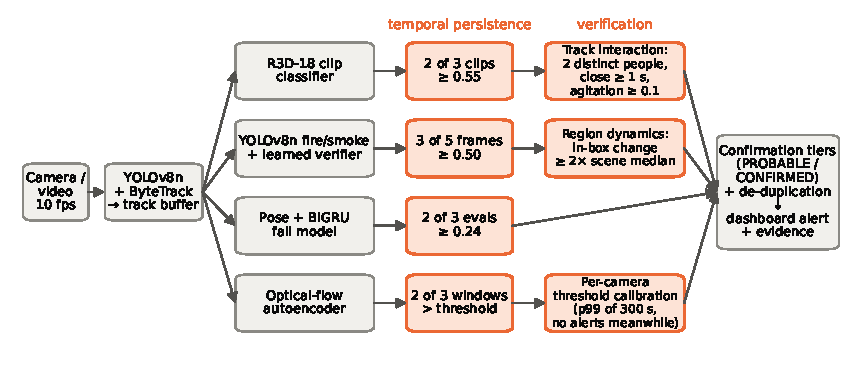
\includegraphics[width=0.9\textwidth]{pipeline.pdf}
\caption{Pipeline. Shaded boxes are the verification stages evaluated in the ablation; thresholds are the deployed configuration.}
\label{fig:pipeline}
\end{figure*}

\subsection{Base detectors}
\textbf{Fight:} R3D-18 on 16-frame clips sampled at 10 frames/s of real time, scored every 4 processed frames when a permissive motion gate is open. \textbf{Fire/smoke:} YOLOv8n fine-tuned on fire/smoke images, followed by a gradient-boosting verifier on flicker, colour, texture and upward-motion features. \textbf{Fall:} YOLOv8n-Pose skeletons and boxes over 4-s windows, classified by a temporal CNN and a bidirectional GRU. \textbf{Unusual activity:} a denoising autoencoder on 38 optical-flow and appearance-change features per 2-s window; the score is reconstruction error divided by a threshold (95th percentile of normal training windows).

\subsection{Temporal persistence}
Each detector alerts only when $N$ of its last $M$ evaluations are positive: 2 of 3 R3D-18 clips at score $\ge 0.55$; 3 of 5 sampled frames at YOLO confidence $\ge 0.50$ for fire/smoke; 2 of 3 fall evaluations; 2 of 3 anomaly windows. A single fire or smoke class must also stay active for 3\,s.

\subsection{Track-level interaction validation (fights)}
When the R3D-18 rule fires, the alert is kept only if the track buffer shows (1) two \emph{distinct} people, i.e.\ tracks seen within the last 1\,s, after dropping a track whose box overlaps an older one with IoU $\ge 0.7$; (2) a pair whose centre distance, normalised by their mean box height, is $\le 1.2$ for at least 1\,s ($\mathit{close\_seconds}$) within the last 3\,s; and (3) agitation of the more active person
\begin{equation}
a = \frac{\lVert(\sigma(r_x),\sigma(r_y))\rVert + \sigma(w) + \sigma(h)}{\operatorname{median}(h)} \ge 0.1,
\end{equation}
where $r$ is the residual of the box centre around a quadratic fit over the 3-s window, and $w,h$ are box width and height. Walking follows a smooth path and leaves little residual. A pair that qualified within the last 2\,s stays valid, because grappling people are often merged into one box.

\subsection{Region dynamics (fire and smoke)}
When a fire or smoke box persists, the median absolute grey-level change of pixels inside the box is compared with that of the rest of the frame. \emph{Flicker} uses frame-to-frame differences over the last 5 evaluated frames. \emph{Growth} compares the current frame with a reference 8--30\,s old. The alarm is kept only if either ratio is at least 2 (noise floor 1 grey level). Sensor noise and auto-exposure changes shift every pixel together and cancel out. The check reuses frames already evaluated, so it adds no delay.

\subsection{Per-camera anomaly calibration}
For its first 300\,s on a camera, the anomaly detector records the error ratio of every window without alerting. It then sets a camera scale equal to the 99th percentile of those ratios, never below 1, and stores it for later restarts.

\section{Experimental Setup}
\subsection{Model evaluation data}
The fight model used 2{,}300 fight and non-fight videos~\cite{akti2019}~\verify{}, split by video into 1{,}612 train, 344 validation and 344 test; thresholds were chosen on validation. The fall models used 160 staged videos (79 falls, 81 non-falls, 48 events) with 5-fold cross-validation grouped by event. The fire verifier used FIRESENSE~\cite{dimitropoulos2015} (27 fire, 22 smoke videos) with leave-one-video-out evaluation. The anomaly autoencoder v2 was tested on 23 unseen normal and 79 abnormal videos, split by event.

\subsection{Ablation data (proxy)}
The study was designed around recordings from the deployment camera (15--30\,min of normal activity, staged events, and fire look-alikes). \textbf{These recordings were not available}, so we built labelled proxy sets from clips already in the project (Table~\ref{tab:sets}). The normal set is the fight test split's not-fight half, on which no deployed model was trained. The proxy differs from the intended study in two ways. Its clips come from many cameras and last a few seconds each. Three sets also overlap model training: the deployed fall model was trained on the fall clips and the fire verifier on FIRESENSE, so recall on those sets is in-sample.

\begin{table}[t]
\caption{Proxy clip sets for the ablation}
\label{tab:sets}
\centering
\footnotesize
\begin{tabular}{lrrl}
\toprule
Set & Clips & Min & Source / note \\
\midrule
Normal & 172 & 16.0 & fight test split, not-fight (no model trained on it) \\
Look-alikes & 25 & 14.8 & FIRESENSE negatives \\
Fight & 172 & 15.2 & fight test split (held out) \\
Fall & 79 & 9.0 & in-sample for the fall model \\
Fire & 11 & 5.6 & FIRESENSE positives (verifier in-sample) \\
Smoke & 13 & 8.8 & FIRESENSE positives (verifier in-sample) \\
\bottomrule
\end{tabular}
\end{table}

Per-camera calibration needs 300\,s of one camera. We pooled the windows the real detector recorded on all 172 not-fight clips of the fight \emph{validation} split (915\,s), disjoint from all evaluation sets, and let the detector's own routine compute the 99th percentile. A 5-s clip yields about one 2-s window after warm-up, so the pool holds 51 windows, just above the minimum of 50. Clips were not concatenated, because scene cuts would themselves look abnormal.

\subsection{Configurations and protocol}
(a) The code before the verification stages (commit \texttt{85315cc\textasciitilde1}, its own configuration); (b) the full system; (c) full without the interaction check; (d) full without region dynamics; (e) full without anomaly calibration; (f) full with every $N$-of-$M$ rule set to 1 of 1 and the 3-s fire/smoke sustain set to 0. (c)--(f) change configuration flags only. Every clip is played separately through the production \texttt{run()} function, with fresh tracker, detector, confirmation and de-duplication state, at the live pace of 10 processed frames/s, because the detectors use wall-clock time. The dashboard and LLM are off, and the demo camera's placeholder zones are removed.

\subsection{Metrics}
\emph{False alarms per hour} = dashboard alarms on normal or look-alike clips $\times 60$ / footage minutes, per event type. \emph{Recall} = event clips with at least one dashboard alarm of the matching type / event clips. All 95\,\% confidence intervals are percentile bootstraps over videos (1{,}000 resamples, fixed seed). For model metrics, intervals are computed only where per-video predictions are stored. Hardware: Intel laptop CPU, NVIDIA RTX 3050 laptop GPU.

\section{Results}
\subsection{Per-model results}
Table~\ref{tab:models} lists the deployed model of each task on its own test protocol. Intervals are given only where per-video predictions are stored. For the fight, fall and verified fire/smoke rows only aggregate counts exist, so no interval is computed and a McNemar test of fight v1 against v2 could not be run. Baselines: the first fight model reached F1 0.85, the box-rule fall detector F1 0.81, and YOLO alone on fire F1 0.87 with 2 false alarms (0 with the verifier; with 27 videos this difference is within the interval).

\begin{table}[t]
\caption{Deployed models on held-out data (95\,\% bootstrap CI where per-video predictions exist)}
\label{tab:models}
\centering
\footnotesize
\setlength{\tabcolsep}{3pt}
\begin{tabular}{llrllll}
\toprule
Task & Model & $n$ & P & R & F1 & AUC \\
\midrule
Fight & R3D-18 v2, 2-of-3 & 344 & 0.94 & 0.97 & 0.96 & 0.99 \\
Fall & Pose+BiGRU (CV) & 160 & 0.86 & 0.94 & 0.90 & 0.96 \\
Fire & YOLO+verifier & 27 & 1.00 & 0.91 & 0.95 & -- \\
Fire & YOLO only & 27 & \makecell[l]{0.83\\{}[0.60,1.00]} & \makecell[l]{0.91\\{}[0.71,1.00]} & \makecell[l]{0.87\\{}[0.70,1.00]} & -- \\
Smoke & YOLO+verifier & 22 & 1.00 & 0.85 & 0.92 & -- \\
Anomaly & Autoencoder v2 & 102 & \makecell[l]{0.96\\{}[0.91,1.00]} & \makecell[l]{0.67\\{}[0.57,0.77]} & \makecell[l]{0.79\\{}[0.71,0.86]} & \makecell[l]{0.84\\{}[0.72,0.93]} \\
\bottomrule
\end{tabular}
\end{table}

\subsection{Ablation}
Table~\ref{tab:ablation} and Fig.~\ref{fig:ablation} give false alarms per hour and recall for each configuration. Table~\ref{tab:paired} gives the paired difference of each configuration against the full system on the same clips. The full system's false alarms on normal clips come mostly from the fall detector (22 of 36), then fights (10), crowds (3) and fire/smoke (1). With calibration on, the anomaly detector raised no alarm on any set. That includes the genuine fire and smoke clips, where it raised 7 and 11 alarms without calibration. The calibrated threshold, from 51 pooled windows, was 8.7$\times$ the model's.

\begin{table*}[t]
\caption{False alarms per hour (FA/h, 95\,\% CI) and clip-level recall on the proxy sets}
\label{tab:ablation}
\centering
\footnotesize
\begin{tabular}{lllllll}
\toprule
Configuration & FA/h normal & FA/h look-alikes & Fight & Fall & Fire & Smoke \\
\midrule
(a) pre-fix code & 157.9 [105.3, 226.9] & 109.5 [72.7, 166.3] & 0.78 & 0.75 & 0.73 & 0.62 \\
(b) full system & 135.3 [81.0, 210.8] & 44.6 [25.4, 69.8] & 0.47 & 0.75 & 0.73 & 0.62 \\
(c) $-$ interaction & 139.1 [85.2, 214.4] & 56.8 [33.6, 86.7] & 0.75 & 0.75 & 0.73 & 0.62 \\
(d) $-$ region dynamics & 135.3 [82.3, 209.8] & 44.6 [25.4, 69.8] & 0.47 & 0.75 & 0.73 & 0.62 \\
(e) $-$ calibration & 146.6 [97.2, 213.5] & 101.3 [69.2, 155.6] & 0.47 & 0.75 & 0.73 & 0.54 \\
(f) single-frame (1/1) & 218.0 [138.1, 326.2] & 77.0 [49.2, 131.4] & 0.48 & 0.91 & 0.91 & 0.85 \\
\bottomrule
\end{tabular}
\end{table*}

\begin{table*}[t]
\caption{Paired difference, configuration minus full system (95\,\% CI). Positive $\Delta$FA: the stage removes false alarms; positive $\Delta$recall: the stage costs detections}
\label{tab:paired}
\centering
\footnotesize
\begin{tabular}{lllllll}
\toprule
Configuration & $\Delta$FA/h normal & $\Delta$FA/h look-alikes & $\Delta$R fight & $\Delta$R fall & $\Delta$R fire & $\Delta$R smoke \\
\midrule
(a) pre-fix & +22.6 [0.0, 41.5] & +64.9 [40.2, 105.8] & +0.31 [0.24, 0.38] & 0 & 0 & 0 \\
(c) $-$ interaction & +3.8 [$-$13.8, 22.3] & +12.2 [0.0, 24.8] & +0.28 [0.21, 0.35] & 0 & 0 & 0 \\
(d) $-$ dynamics & 0.0 [$-$11.2, 11.4] & 0.0 & $-$0.01 [$-$0.02, 0.00] & 0 & 0 & 0 \\
(e) $-$ calibration & +11.3 [$-$9.2, 29.8] & +56.8 [35.3, 96.3] & $-$0.01 [$-$0.03, 0.02] & 0 & 0 & $-$0.08 [$-$0.23, 0.00] \\
(f) single-frame & +82.7 [44.7, 135.9] & +32.4 [11.8, 70.8] & +0.01 [$-$0.01, 0.04] & +0.16 [0.09, 0.24] & +0.18 [0.00, 0.45] & +0.23 [0.00, 0.46] \\
\bottomrule
\end{tabular}
\end{table*}

\begin{figure*}[t]
\centering
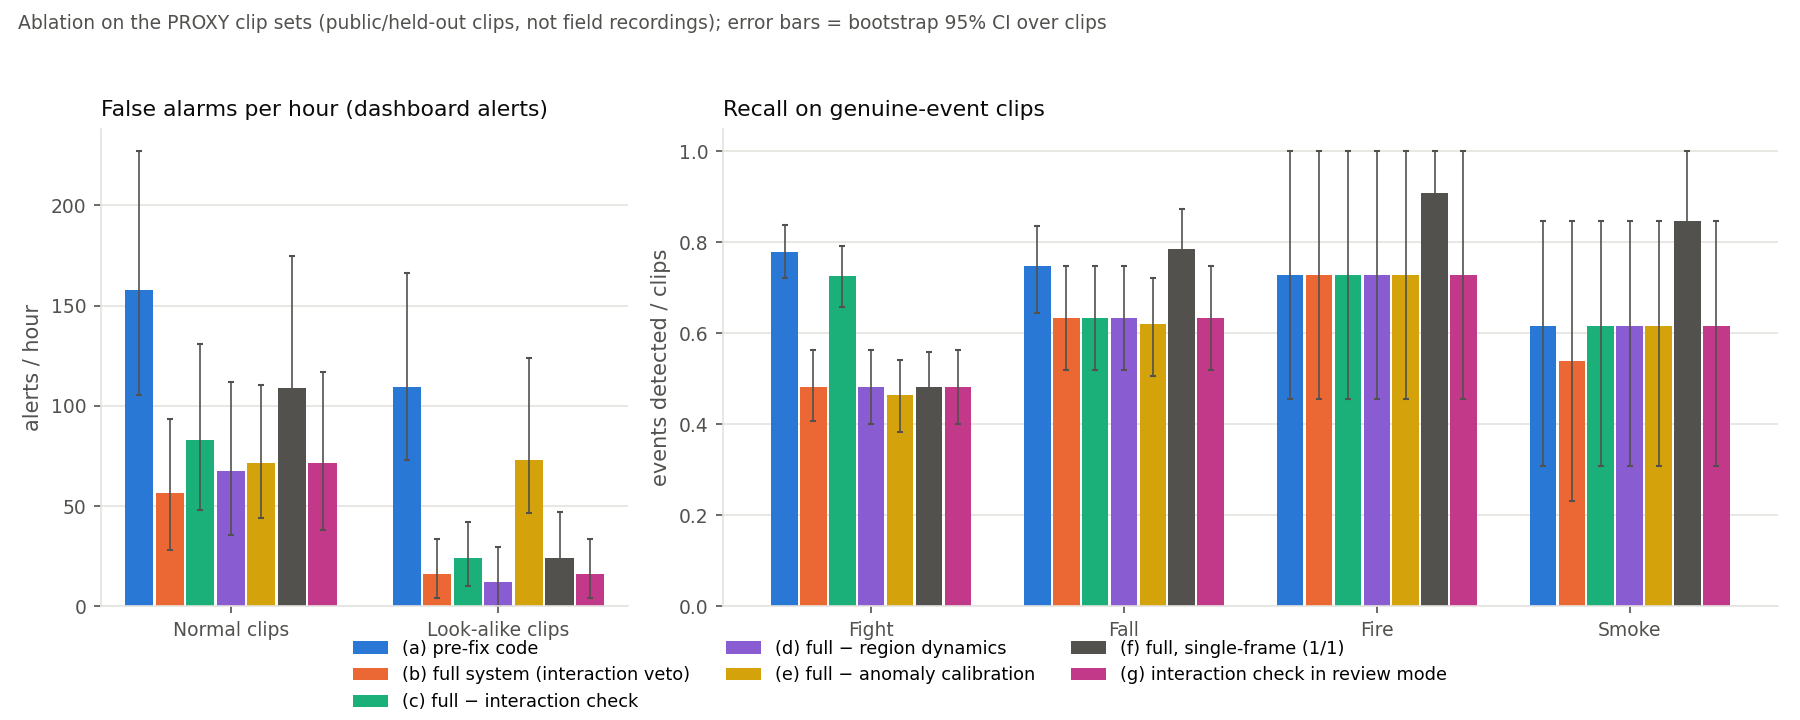
\includegraphics[width=0.95\textwidth]{ablation.png}
\caption{False alarms per hour (left) and recall (right) per configuration on the proxy sets; error bars are 95\,\% bootstrap CIs.}
\label{fig:ablation}
\end{figure*}

\subsection{Fight interaction thresholds}
On the 344 held-out fight-test clips, a pair stayed close for at least 1\,s in 51\,\% of fight clips and 51\,\% of normal clips. The agitation of a close pair separated the classes with ROC AUC 0.55 [0.50, 0.61] (Fig.~\ref{fig:interaction}). At the configured 0.1, 51\,\% of fight and 42\,\% of normal clips pass (Youden $J$ 0.08 [$-$0.02, 0.19]). At 0.2, the best value on these clips, 47\,\% and 29\,\% pass ($J$ 0.17 [0.08, 0.28]). The paired gain in $J$ is [0.04, 0.15], but it was selected on the same clips.

\begin{figure}[t]
\centering
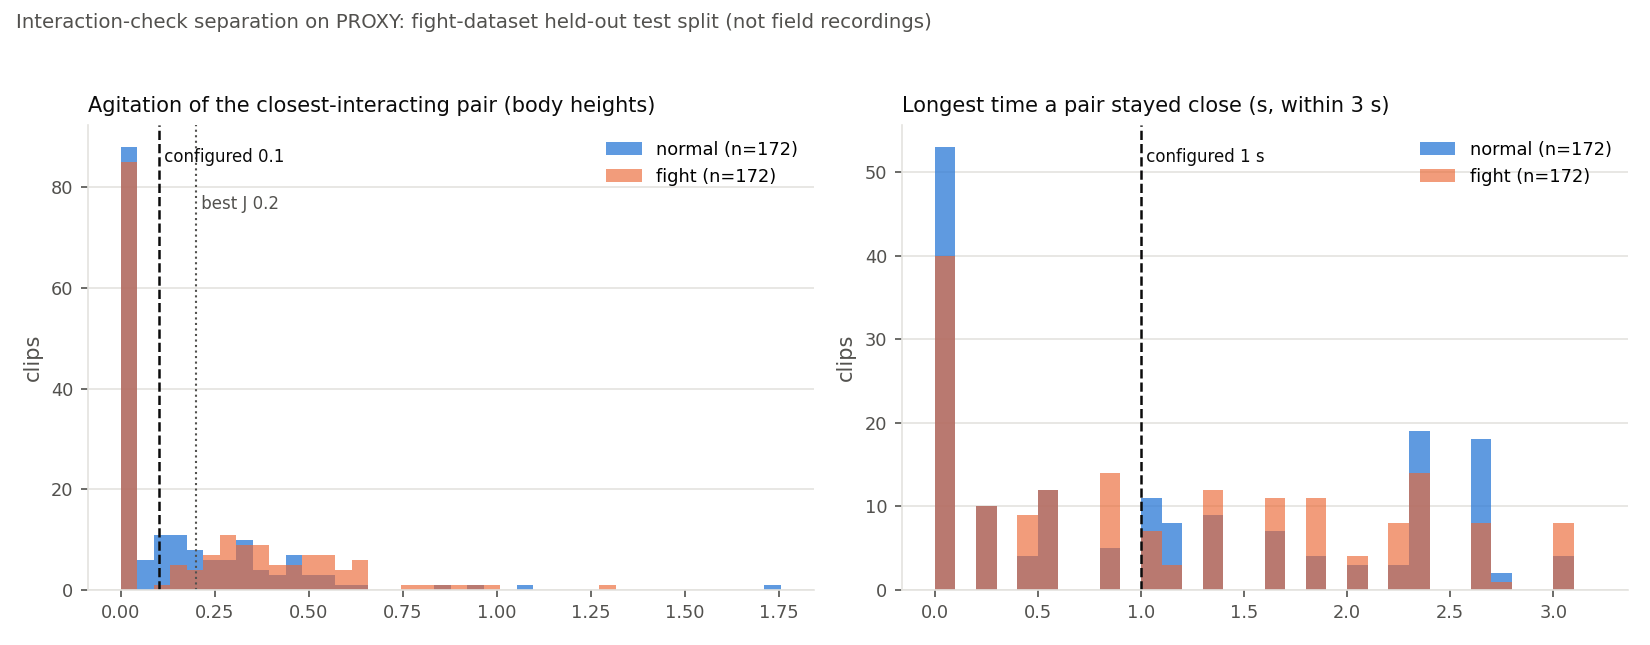
\includegraphics[width=\columnwidth]{interaction_separation.png}
\caption{Agitation of the closest-interacting pair (left) and longest close time (right), fight vs normal clips.}
\label{fig:interaction}
\end{figure}

\subsection{Speed}
On the RTX 3050 laptop GPU the whole pipeline takes 51.9\,ms per frame and sustains 9.2 of the 10 target frames/s (capacity 19.3). On the CPU it takes 153.8\,ms and sustains 6.1 frames/s. The fight stage, including the interaction check, adds 7.2\,ms per frame on the GPU.

\section{Discussion}
\textbf{Persistence does most of the work, and is a real trade-off.} Requiring $N$ of $M$ positive windows removes 82.7 false alarms per hour on normal clips and 32.4 on look-alikes. It costs 0.16 fall recall, and the fire and smoke losses are of similar size, though their intervals reach zero. It is cheap and transparent, and $N$ and $M$ are the natural knob to tune per site.

\textbf{A hard gate on weak evidence hurts recall.} The interaction check encodes a physically sensible requirement, but its inputs come from a tracker that often merges grappling people or loses them in crowded, low-resolution clips. Half of the held-out fight clips never showed a close pair. A check that can only veto should not depend on evidence missing half the time. The agitation feature carries some signal, so it may work better as a soft confidence term or a review flag.

\textbf{Calibration fixes false alarms by moving the threshold, possibly too far.} Calibration removed every unusual-activity false alarm, but at 8.7$\times$ the model's threshold it also removed every detection we could observe. In the proxy it pooled 51 windows from 172 different cameras, so the 99th percentile mixes scene types. On one fixed camera, the deployed design, the spread of normal scores should be narrower. Whether calibration then preserves detections is the most important open measurement.

\textbf{Some verification is untestable with public data.} FIRESENSE negatives never triggered the fire detector, so region dynamics could not act. The null result says nothing about the stage, only about the test data.

\textbf{Implication.} The claim holds for look-alike scenes: false alarms fall by 64.9 per hour with fall, fire and smoke recall unchanged. It does not hold for fights, where recall falls by 0.31. On normal clips the reduction is not distinguishable from zero. Unit tests of the targeted failure passed for all four stages, yet one failed end to end. A verification stage should be accepted only with an end-to-end recall measurement.

\section{Limitations}
\begin{itemize}
\item \textbf{Proxy data.} No deployment-camera footage was available. The clips are short and come from many cameras, so per-hour rates are rates on other people's cameras, and per-camera calibration had to be pooled across cameras.
\item \textbf{In-sample sets.} Fall recall is in-sample for the fall model, and fire/smoke recall for the fire verifier.
\item \textbf{Single runs.} Each configuration was run once. The pipeline is timing-dependent, so a re-run can differ by an alert or a detection.
\item \textbf{Small sets.} The fire (11) and smoke (13) event sets give wide intervals.
\item \textbf{No unusual-activity event set.} Calibration's cost in anomaly recall is seen only indirectly, as alarms on other event clips.
\item \textbf{Missing intervals.} Fight, fall and verified fire/smoke metrics store only aggregate counts, so they have no interval and no paired significance test.
\end{itemize}

\section{Conclusion}
We ablated four verification stages of a multi-event CCTV pipeline end to end, in real time and on unchanged production code. On held-out and public clips, the stages cut false alarms on fire look-alike scenes by more than half, mainly through persistence and anomaly calibration. They did not keep fight recall: the track-level interaction check removed more true fights than false ones. Calibration also silenced the anomaly detector, and the look-alike check could not be exercised. The protocol, scripts and per-clip outcomes are released with the system. They switch to field recordings when these exist; the next step is the same ablation on the deployment camera's own footage.

\begin{thebibliography}{99}
\bibitem{redmon2016} J. Redmon, S. Divvala, R. Girshick, and A. Farhadi, ``You Only Look Once: Unified, real-time object detection,'' in \emph{Proc. CVPR}, 2016.
\bibitem{yolov8} G. Jocher, A. Chaurasia, and J. Qiu, \emph{Ultralytics YOLOv8}, software, 2023. [Online]. Available: \url{https://github.com/ultralytics/ultralytics}
\bibitem{zhang2022} Y. Zhang \emph{et al.}, ``ByteTrack: Multi-object tracking by associating every detection box,'' in \emph{Proc. ECCV}, 2022.
\bibitem{tran2018} D. Tran, H. Wang, L. Torresani, J. Ray, Y. LeCun, and M. Paluri, ``A closer look at spatiotemporal convolutions for action recognition,'' in \emph{Proc. CVPR}, 2018.
\bibitem{kay2017} W. Kay \emph{et al.}, ``The Kinetics human action video dataset,'' arXiv:1705.06950, 2017.
\bibitem{cheng2021} M. Cheng, K. Cai, and M. Li, ``RWF-2000: An open large scale video database for violence detection,'' in \emph{Proc. ICPR}, 2021. \verify{} (arXiv 2019; ICPR 2020 published 2021)
\bibitem{akti2019} \c{S}. Akt\i, G. A. Tataro\u{g}lu, and H. K. Ekenel, ``Vision-based fight detection from surveillance cameras,'' in \emph{Proc. IPTA}, 2019. \verify{}
\bibitem{selvaraju2017} R. R. Selvaraju \emph{et al.}, ``Grad-CAM: Visual explanations from deep networks via gradient-based localization,'' in \emph{Proc. ICCV}, 2017.
\bibitem{hasan2016} M. Hasan, J. Choi, J. Neumann, A. K. Roy-Chowdhury, and L. S. Davis, ``Learning temporal regularity in video sequences,'' in \emph{Proc. CVPR}, 2016.
\bibitem{sultani2018} W. Sultani, C. Chen, and M. Shah, ``Real-world anomaly detection in surveillance videos,'' in \emph{Proc. CVPR}, 2018.
\bibitem{celik2009} T. \c{C}elik and H. Demirel, ``Fire detection in video sequences using a generic color model,'' \emph{Fire Safety J.}, vol. 44, no. 2, 2009.
\bibitem{dimitropoulos2015} K. Dimitropoulos, P. Barmpoutis, and N. Grammalidis, ``Spatio-temporal flame modeling and dynamic texture analysis for video-based fire detection,'' \emph{IEEE Trans. Circuits Syst. Video Technol.}, 2015. \verify{}
\bibitem{maji2022} D. Maji, S. Nagori, M. Mathew, and D. Poddar, ``YOLO-Pose: Enhancing YOLO for multi person pose estimation using object keypoint similarity loss,'' in \emph{Proc. CVPR Workshops}, 2022.
\bibitem{cho2014} K. Cho \emph{et al.}, ``Learning phrase representations using RNN encoder--decoder for statistical machine translation,'' in \emph{Proc. EMNLP}, 2014.
\end{thebibliography}

\end{document}
